\documentclass[a4paper]{article}

\usepackage{Template}

%标题部分
\title{\LaTeX 模板}
\author{JamesZhutheThird}
\date{\today}
%\date{YYYYMMDD}

\begin{document}

\thispagestyle{fancy}
\maketitle

%摘要部分
\begin{abstract}
摘要摘要摘要摘要摘要摘要摘要摘要摘要摘要摘要摘要摘要摘要摘要摘要摘要摘要摘要摘要摘要摘要摘要摘要摘要摘要\textbf{关键字}摘要摘要摘要摘要摘要摘要摘要摘要摘要摘要摘要摘要摘要摘摘要摘要摘要摘要摘要摘要摘要摘要摘要摘要摘要摘要摘要摘要要摘要摘要摘要摘要摘要摘要摘要摘要摘要摘要摘要摘要摘要摘要摘要摘要\textbf{关键字}摘要摘要摘要摘要摘要摘要摘要摘要摘要摘要\textbf{关键字}摘要摘要摘要摘要摘要摘要摘要\textbf{关键字}摘要摘要摘要摘要摘要摘要摘要摘要摘要摘要摘要摘要摘要摘要摘要摘要摘要
\par\textbf{关键字:}关键字,关键字,关键字,关键字
\end{abstract}


\section{模板}
\subsection{插入图片}
\subsubsection{单张图片}
正文正文正文正文正文正文正文正文正文正文正文正文正文正文正文正文正文正文正文正文正文正文正文正文正文正文正文正文正文正文正文正文正文正文正文正文正文正文正文正文正文正文正文正文正文正文正文正文正文正文正文正文正文正文正文正文正文正文正文正文正文正文正文正文正文正文正文正文正文正文正文正文如图\ref{fig1}所示

\begin{figure}[!h]
	\centering
	\vspace{0cm}
	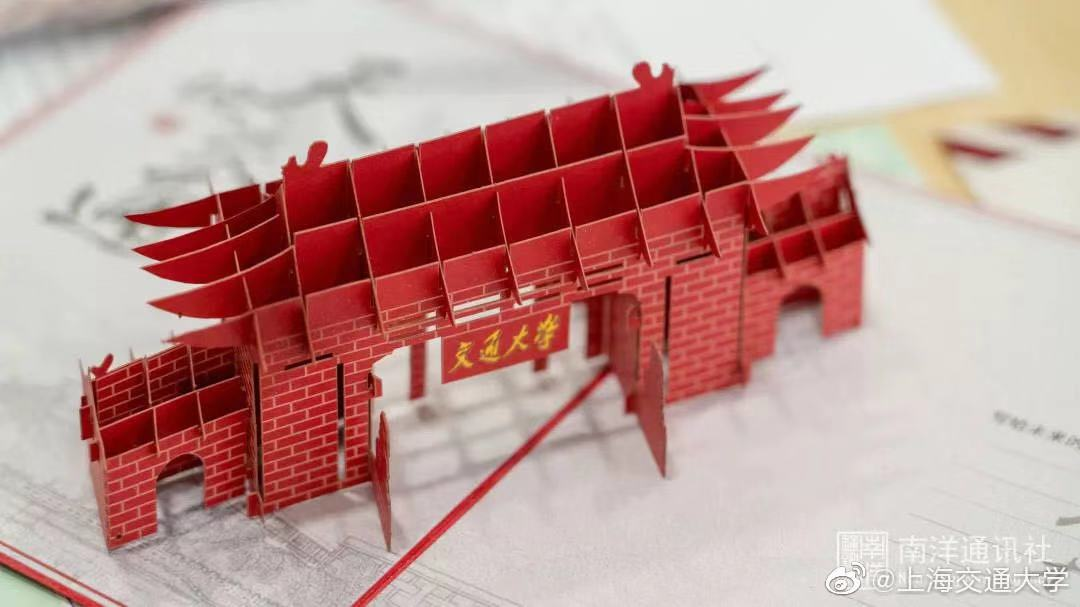
\includegraphics[width=0.7\textwidth,trim=50 100 200 75,clip]{figures/fig1.jpg}%trim裁切依次左下右上
	\vspace{0cm}
	\caption{图标题}
	\label{fig1}
\end{figure}

\subsubsection{多张图片}
正文正文正文正文正文正文正文正文正文正文正文正文正文正文正文正文正文正文正文正文正文正文正文正文正文正文正文正文正文正文正文正文正文正文正文正文正文正文正文正文正文正文正文正文正文正文正文正文正文正文正文正文正文正文正文正文正文正文正文正文正文正文正文正文正文正文正文正文正文正文正文正文如图\ref{fig2}所示

\begin{figure}[!h]
	\centering
	\subfigure[子图1标题]{
		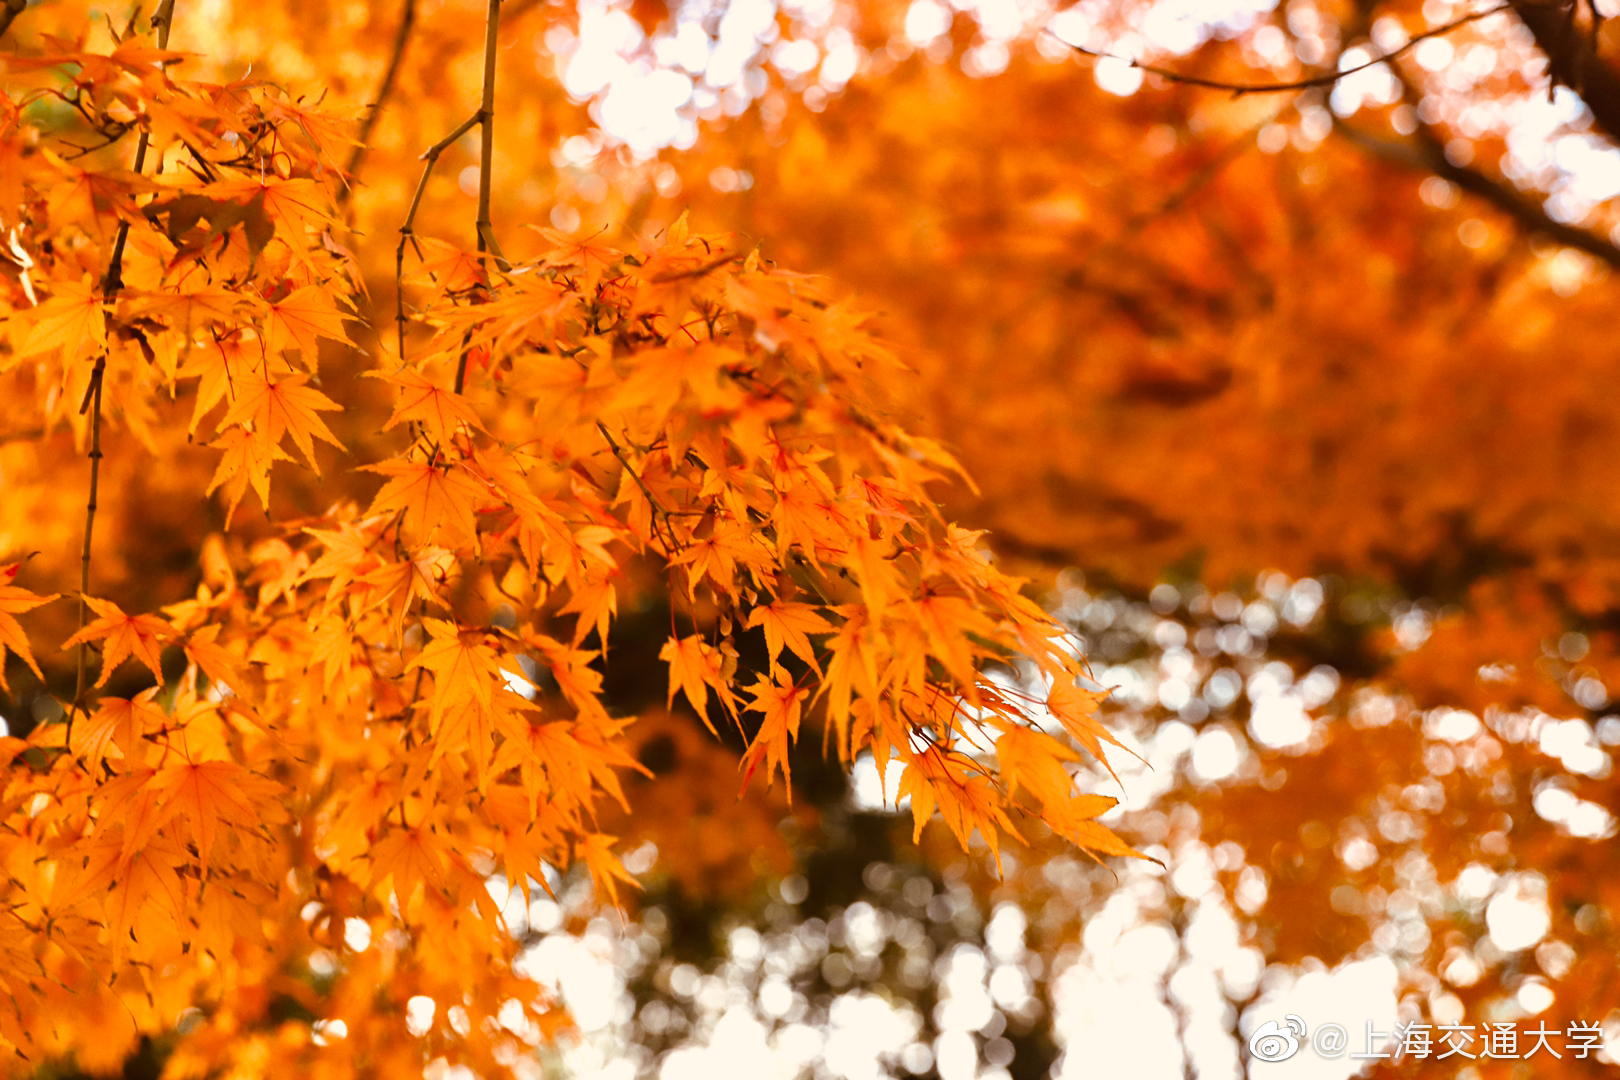
\includegraphics[width=0.2\linewidth,trim=0 0 0 0,clip]{figures/fig2-1.jpg}}%trim裁切依次左下右上
	\subfigure[子图2标题]{
		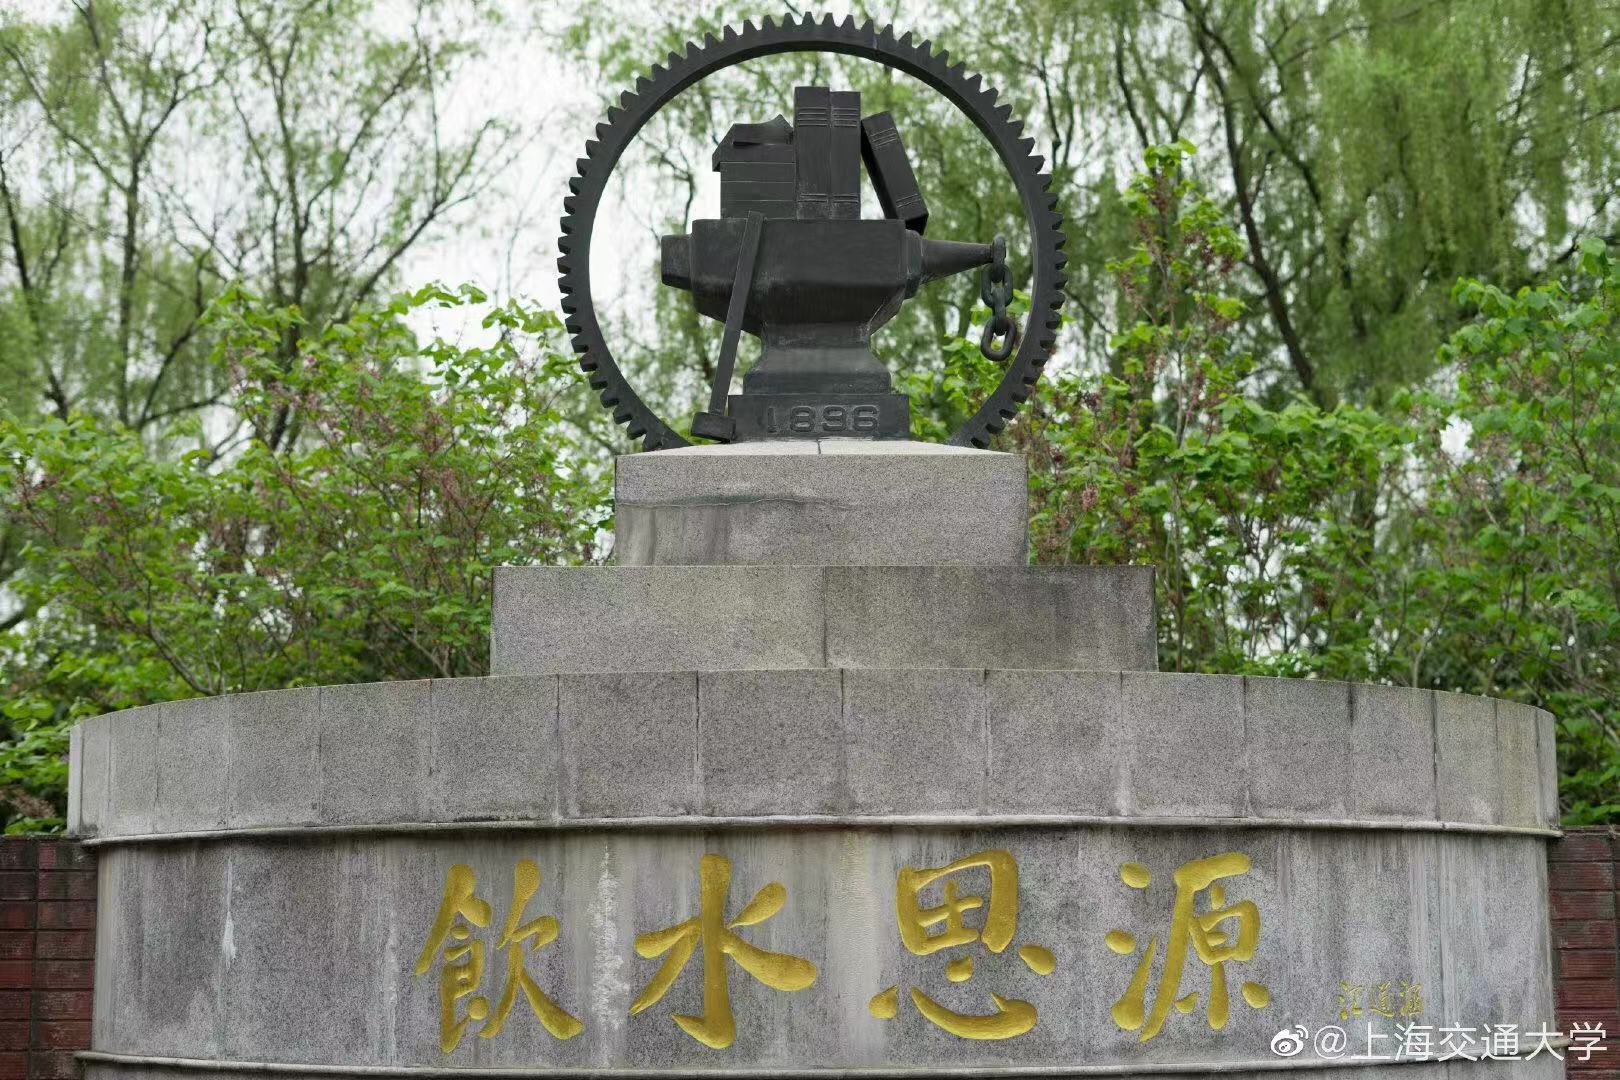
\includegraphics[width=0.2\linewidth,trim=0 0 0 0,clip]{figures/fig2-2.jpg}}%trim裁切依次左下右上
	\subfigure[子图3标题]{
		\includegraphics[width=0.2\linewidth,trim=0 0 0 0,clip]{figures/fig2-3.jpg}}%trim裁切依次左下右上
	\subfigure[子图4标题]{
		\includegraphics[width=0.2\linewidth,trim=0 0 0 0,clip]{figures/fig2-4.jpg}}%trim裁切依次左下右上
	\caption{图标题}
	\label{fig2}
\end{figure}
%多图并列换行自动,可用空格\quad等控制

\subsection{插入公式}
正文正文正文正文正文正文正文正文正文正文正文正文正文正文正文正文正文正文正文正文正文正文正文正文正文正文正文正文正文正文正文正文正文正文正文正文正文正文正文正文\textbf{行内公式}$1+1=2$正文正文正文正文正文正文正文正文正文正文正文正文正文正文正文正文正文正文正文正文正文正文正文正文正文正文正文正文正文正文正文正文

行间公式
$$
1-1=0
$$

更复杂的带序号行间公式见\ref{formula}
\begin{equation}
\begin{aligned}
1*1&=1\\
1/1&=1
\end{aligned}
\label{formula}
\end{equation}

完整公式汇总参见\url{https://1024th.github.io/MathJax_Tutorial_CN/#/document}

\subsection{插入表格}

\begin{table}[!h]
\centering
\begin{tabular}{ccccccc}
\toprule

\multirow{2.5}{*}{模型}&\multicolumn {3}{c}{训练集}&\multicolumn {3}{c}{开发集} \\

\cmidrule(r){2-4}\cmidrule(r){5-7}
&ACC&AUC&EER&ACC&AUC&EER  \\
\midrule
GMM_{3}^{13}&$0.9592$&$0.9393$&$0.0926$&$0.9596$&$0.9400$&$0.0911$\\    
GMM_{6}^{13}&$0.9620$&$0.9506$&$0.0676$&$0.9623$&$0.9516$&$0.0654$\\ 
GMM_{9}^{13}&$0.9659$&$0.9562$&$0.0592$&$0.9661$&$0.9564$&$0.0590$\\ 
GMM_{12}^{13}&$0.9654$&$0.9543$&$0.0635$&$0.9654$&$0.9535$&$0.0646$\\ 
GMM_{15}^{13}&$0.9654$&$0.9540$&$0.0641$&$0.9657$&$0.9551$&$0.0617$\\ 
GMM_{18}^{13}&$0.9661$&$0.9560$&$0.0602$&$0.9661$&$0.9559$&$0.0603$\\ 
\midrule
EGMM_{3}^{13}&$0.9572$&$0.9474$&$0.0682$&$0.9569$&$0.9474$&$0.0677$\\    
EGMM_{6}^{13}&$0.9621$&$0.9541$&$0.0587$&$0.9626$&$0.9553$&$0.0561$\\ 
EGMM_{9}^{13}&$0.9632$&$0.9583$&$0.0495$&$0.9632$&$0.9585$&$0.0490$\\                         
EGMM_{12}^{13}&$0.9619$&$0.9612$&$0.0399$&$0.9615$&$0.9604$&$0.0413$\\ 
EGMM_{15}^{13}&$0.9629$&$0.9609$&$0.0423$&$0.9629$&$0.9606$&$0.0430$\\ 
EGMM_{18}^{13}&$0.9630$&$0.9609$&$0.0425$&$0.9628$&$0.9606$&$0.0430$\\ 
\bottomrule
\end{tabular}
\label{wexample}
\vspace{-15pt}
\caption{改变高斯分量数量结果对比}
\end{table}

\section*{备注}
%Licence 请勿删除
本文排版基于\LaTeX{}\href{https://cn.overleaf.com/read/mxmypkyfrzpz}{【OverLeaf】}\href{https://latex.sjtu.edu.cn/read/ndjrkpksrfzn}{【SJTU-ShareLatex】}模板,采用\href{http://creativecommons.org/licenses/by-nc-sa/4.0/}{【CC BY-NC-SA 4.0】}进行许可。


\bibliographystyle{unsrt}
\bibliography{cite}

\section*{附录}
\subsection*{MATLAB代码}
\lstinputlisting{demo.m}


\end{document}
